\documentclass[letterpaper,twocolumn,10pt]{article}
\usepackage{usenix2019_v3}

% to be able to draw some self-contained figs
\usepackage{tikz}
\usepackage{amsmath}
\usepackage{graphicx}
\usepackage{comment}

\graphicspath{ {./images/} }

%-------------------------------------------------------------------------------
\begin{document}
%-------------------------------------------------------------------------------

%don't want date printed


% make title bold and 14 pt font (Latex default is non-bold, 16 pt)
\title{\Large \bf Density Based Clustering for Hierarchical and Autonomous Fog Architecture}


%for single author (just remove % characters)
\author{
{\rm Robin C.\ Ward}\\
PhD Student\\
Auburn University\\
Auburn, Alabama 36849\\
Email: rcw0024@auburn.edu\\
Last Edit: \today
} % end author

\maketitle

%-------------------------------------------------------------------------------
\begin{abstract}
%-------------------------------------------------------------------------------
Our population is increasing rapidly(there is approximately a net gain of one new person on the planet Earth every 31 seconds\footnote{\url{https://www.census.gov/popclock}}), and the need to manage all of those new devices coming online will grow with it. Thankfully, HAFA~\cite{10.1145/3229710.3229740} was designed to handle such situations. However, when given a finite resource such as the space on planet Earth, and combine that with a growing population, clustering based on density will be very important. This paper will cover the implementation of other clustering algorithms, such as the DBSCAN~\cite{10.5555/3001460.3001507} method, into the HAFA architecture.

I am currently exploring the idea of:
As an initial pass would greatly reduce the overall average case run time.
\end{abstract}


%-------------------------------------------------------------------------------
\section{Introduction}
%-------------------------------------------------------------------------------

The following sections are part of a hypothesis. No tests have been completed yet, so there are currently no test results.


\subsection{Proposed changes to HAFA}
\begin{description}
\item[Use DBSCAN on first pass.] Use DBSCAN to cluster highly dense areas within each layer. This will enable DBSCAN to cluster nodes in highly dense areas very fast, then cluster the outliers based on the Agglomerative Complete Linkage Hierarchical Clustering method. The use of DBSCAN could be based on several factors, including but not limited to: distance, MIPS, power. For example, the radius of the circle for the Core Point~\ref{fig:pseudocode} qualification could increase for a specific node if they are lacking certain resources and require more for specific load balancing activities.

\item[Finding a value for Epsilon.] Perhaps for the specific fog layer or data set that is being used, some kind of check could be performed to see if the average MIPS of the nodes are at a threshold. For example, if the average MIPS are not meeting the threshold, the Epsilon for DBSCAN could increase in an effort to make larger clusters. These larger clusters would allow for better load balancing due to the increased amount of hardware. Some quick pseudo-code could be:
\begin{verbatim}
# Finding a value for DBSCAN(Eps)
if AverageMIPS < threshold:
 return .3
else:
 return .2
\end{verbatim}
 The return values need work...perhaps a loop to keep increasing until the average MIPS is no longer below the threshold. This would require a different idea. This would involve a loop that checks the current MIPS within the cluster as DBSCAN runs, then if they do not meet the threshold, the Eps could increase in size to acquire more nodes. Another idea: have the MIPS per cluster be a new variable within HAFA. Then, as DBSCAN runs, it will check if it has hit that threshold, if yes, then the MinPts and Eps could drastically change so that the current clustering process ends, thus forming a new cluster.
 
 \item[Using Great-circle distance vs. Euclidean.] Because earth is mostly spherical, if using a distance metric for geographic data, it would make more sense to use Great-circle distance.
\end{description}

\subsection{Potential Problems and Solutions}
This section covers possible issues that will arise during testing, as well as possible solutions.
\begin{description}
\item[DBSCAN Qualifications.] The use of DBSCAN as a first pass should only be used if it will increase the run time. Therefore, a potential check could be implemented to ensure that running DBSCAN will in fact help with the run time. For example, a city block that only has 10 devices which are spread out could have a longer run time if using the aforementioned method. However, if that same city block had 1000 devices that were tightly packed, the run time would be greatly reduced by using DBSCAN first. Because of this, a qualification algorithm could be implemented to check if DBSCAN would be beneficial or not. Obviously the run time of this check would also have to be low enough to make it worth it. Otherwise, we would just blindly run the DBSCAN every time, which could still be the better option. An example qualification algorithm could be:
\begin{verbatim}
if point_density > threshold:
 return DBSCAN + Agglomerative
else:
 return Agglomerative
\end{verbatim}
An important item to note here is there is an existing algorithm within the DBSCAN paper that covers getting Epsilon. This could potentially be used for finding the point density for the "precheck".
\end{description}

\subsection{Computational Complexity of using DBSCAN within HAFA}

\begin{description}
\item[Best-case] Best case complexity should be $O (n log n)$ vs. $O(n^3)$ of HAFA.
\item[Average-case] Average case complexity should be better.
\item[Worst-case] Worst-case complexity should remain the same as HAFA, $O(n^3)$.

\end{description}





\begin{figure}[h]
\centering
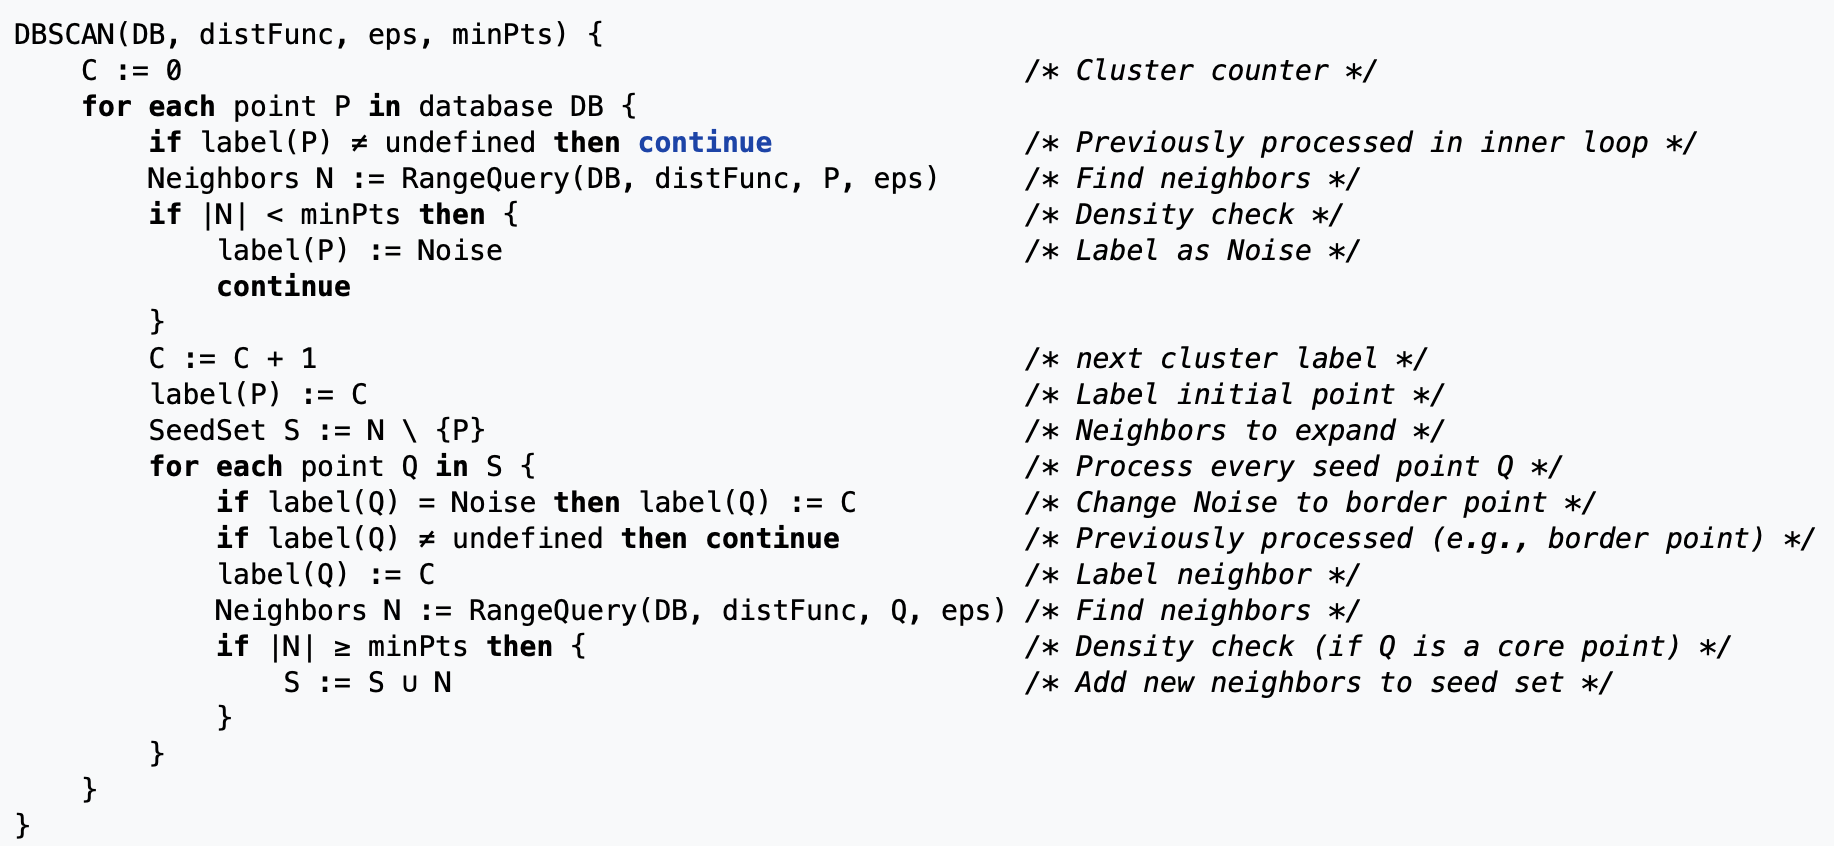
\includegraphics[width=0.45\textwidth]{pseudocode}
\caption{\label{fig:pseudocode}DBSCAN Pseudocode.}
\end{figure}

\bibliographystyle{plain}

\bibliography{bibliography.bib}
%%%%%%%%%%%%%%%%%%%%%%%%%%%%%%%%%%%%%%%%%%%%%%%%%%%%%%%%%%%%%%%%%%%%%%%%%%%%%%%%
\end{document}
%%%%%%%%%%%%%%%%%%%%%%%%%%%%%%%%%%%%%%%%%%%%%%%%%%%%%%%%%%%%%%%%%%%%%%%%%%%%%%%%

%%  LocalWords:  endnotes includegraphics fread ptr nobj noindent
%%  LocalWords:  pdflatex acks